\documentclass[12pt,a4paper]{article}
\usepackage[utf8]{inputenc}
\usepackage[finnish]{babel}
\usepackage{setspace}
%\usepackage{parskip}
%\usepackage{amssymb}
%\usepackage{amsmath}
\usepackage{graphicx}
\usepackage{subcaption}
\usepackage{fancyhdr}
\usepackage[top=1in, bottom=1in, left=1in, right=1in]{geometry}
\usepackage{float}
\usepackage[section]{placeins}
\usepackage[nottoc,notlot,notlof]{tocbibind}
\usepackage{fixltx2e}

\usepackage{titlesec}
\titleclass{\section}{top}
\newcommand\sectionbreak{\clearpage}
\titleformat*{\section}{\Huge\bfseries}
\titleformat*{\subsection}{\Large\bfseries}
\titleformat*{\subsubsection}{\large\bfseries}

%\usepackage[numbered,autolinebreaks,useliterate]{mcode}

\usepackage{siunitx}\sisetup{per=frac} % SI-yksiköitä.
%\usepackage{supertabular} % jos tarttee isoja taulukoita

\usepackage{hyperref}
\hypersetup{pdfborder={0 0 0}}
\onehalfspacing
\cfoot{}
\setlength{\parindent}{0pt}
\newcommand{\yt}{\texttt{yt}}

% pythonjutut
\usepackage{color}
\usepackage{listings}
\usepackage{setspace}

\definecolor{Code}{rgb}{0,0,0}
\definecolor{Decorators}{rgb}{0.5,0.5,0.5}
\definecolor{Numbers}{rgb}{0.5,0,0}
\definecolor{MatchingBrackets}{rgb}{0.25,0.5,0.5}
\definecolor{Keywords}{rgb}{0,0,1}
\definecolor{self}{rgb}{0,0,0}
\definecolor{Strings}{rgb}{0,0.63,0}
\definecolor{Comments}{rgb}{0,0.63,1}
\definecolor{Backquotes}{rgb}{0,0,0}
\definecolor{Classname}{rgb}{0,0,0}
\definecolor{FunctionName}{rgb}{0,0,0}
\definecolor{Operators}{rgb}{0,0,0}
\definecolor{Background}{rgb}{0.98,0.98,0.98}

\lstset{
  literate={ö}{{\"o}}1
           {ä}{{\"a}}1
           {ü}{{\"u}}1
}
\lstdefinestyle{python}{
numbers=left,
numberstyle=\footnotesize,
numbersep=1em,
xleftmargin=1em,
framextopmargin=2em,
framexbottommargin=2em,
showspaces=false,
showtabs=false,
showstringspaces=false,
frame=l,
tabsize=4,
% Basic
basicstyle=\ttfamily\small\setstretch{1},
backgroundcolor=\color{Background},
language=Python,
% Comments
commentstyle=\color{Comments}\slshape,
% Strings
stringstyle=\color{Strings},
morecomment=[s][\color{Strings}]{"""}{"""},
morecomment=[s][\color{Strings}]{'''}{'''},
% keywords
morekeywords={import,from,class,def,for,while,if,is,in,elif,else,not,and,or,print,break,continue,return,True,False,None,access,as,,del,except,exec,finally,global,import,lambda,pass,print,raise,try,assert},
keywordstyle={\color{Keywords}\bfseries},
% additional keywords
morekeywords={[2]@invariant},
keywordstyle={[2]\color{Decorators}\slshape},
emph={self},
emphstyle={\color{self}\slshape},
breaklines=true,
breakatwhitespace=true
postbreak=\raisebox{0ex}[0ex][0ex]{\ensuremath{\color{red}\hookrightarrow\space}}
}
%\renewcommand{\lstlistingname}{Uusinimi} %TODO mieti tämä


\begin{document}

% Sisällysluettelo
\newpage
\thispagestyle{empty}
\tableofcontents
\newpage
\setcounter{page}{1}
\parskip=1em \advance\parskip by 0pt plus 2pt
\pagestyle{fancy}
\cfoot{\thepage}

%%%%%%%%%%%%%%% Oleellinen sisältö alkaa%%%%%%%%%%%%%%%
\section{Johdanto}
%TODO http://arxiv.org/pdf/astro-ph/0403044v1.pdf hyvä soossi?

\section{Enzo}
Enzo on astrofysikaalisten fluidien simulointiin käytettävä ilmainen ja avoin simulaatiokoodi, joka on suunniteltu kosmologisten rakenteiden simulointiin. Se tukee muun muassa hydrodynamiikkaa, ideaalista ja epäideaalista magnetohydrodynamiikkaa, N kappaleen simulaatioita, kaasupilvien kemiaa, säteilynkuljetusta, tähtien syntyä sekä maailmankaikkeuden laajenemista. \cite{enzo} %TODO tukeminen tyhmästi sanottu

Enzo hyödyntää mukautuvaa hilantihennystä (\textit{Adaptive Mesh Refinement}, AMR), joka mahdollistaa aika- ja paikkaresoluution kasvattamisen simulaation kiinnostavilla alueilla. Tämä on tärkeää, sillä usein melko pienellä alueella tarvitaan suurta resoluutiota, mutta koko simulaation ajaminen näin suurella tarkkuudella veisi kohtuuttoman paljon aikaa. Kullekin paikalle valitaan sopiva resoluutio automaattisesti käyttäjän määrittelemien ehtojen mukaan. \cite{enzo}

\subsection{Hila}
Simuloitava alue katetaan kokonaan hilalla, jonka tiheys valitaan sellaiseksi, että saavutetaan pienin haluttava resoluutio. Tämä niinkutsuttu juurihila toimii juurena muiden hilojen muodostamalle hierarkialle, joka muodostuu, kun juurihilasta valitaan alueita simuloitavaksi korkeammalla resoluutiolla.\cite{enzo}
	
Kaikki hilat ovat karteesisia ja suorakulmaisia. Alueille, joilla tarvitaan korkeampaa resoluutiota, asetetaan juurihilan kanssa päällekkäin toinen, hienompi hila. Näitä sisäkkäisiä hiloja voi tarvittaessa olla teoriassa mielivaltaisen monta. Kuvassa \ref{fig:enzogrid} on selvästi nähtävillä hilojen mukauttaminen tutkittavaan alueeseen: tiheillä tai muuten kiinnostavilla alueilla kätetään pienempiä ja tiheämpiä hiloja. \cite{enzo} %TODO oikeasti mielivaltaisen monta?
%Alueet, joilla käytetään suurempaa resoluutiota, valitaan siten, että niiden kaikki tahkot ovat päällekäin jonkin matalamman resoluution hilan tahkojen kanssa. 

\begin{figure}
   \centering
   \begin{subfigure}[b]{0.45\textwidth}
       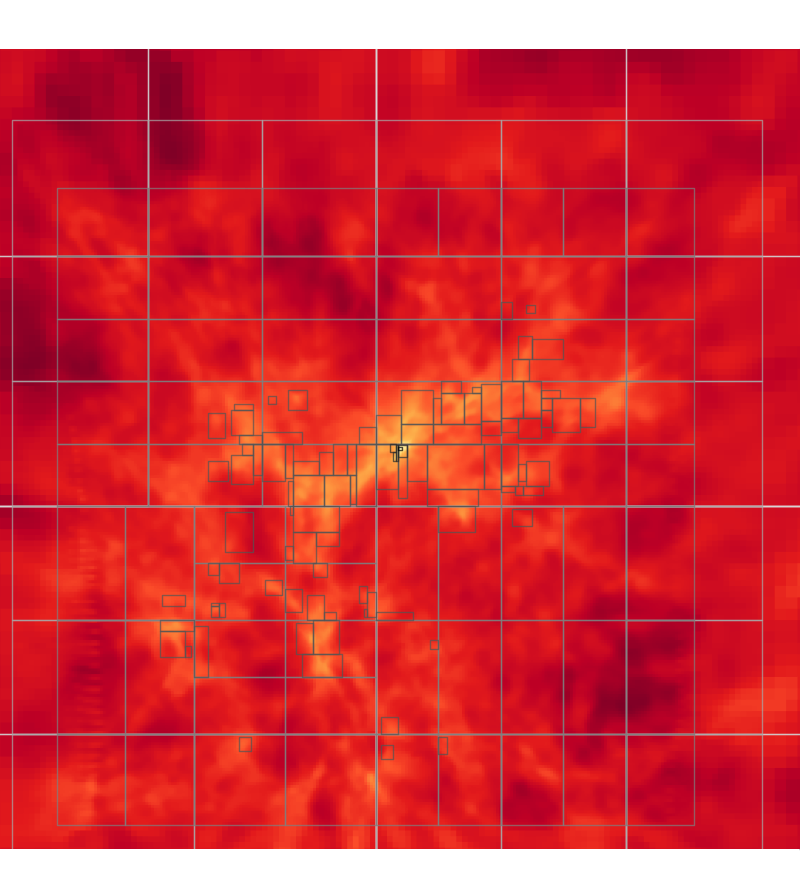
\includegraphics[height=7.9cm]{../kuvat/amr-grid.png}
   \end{subfigure}
   \begin{subfigure}[b]{0.45\textwidth}
       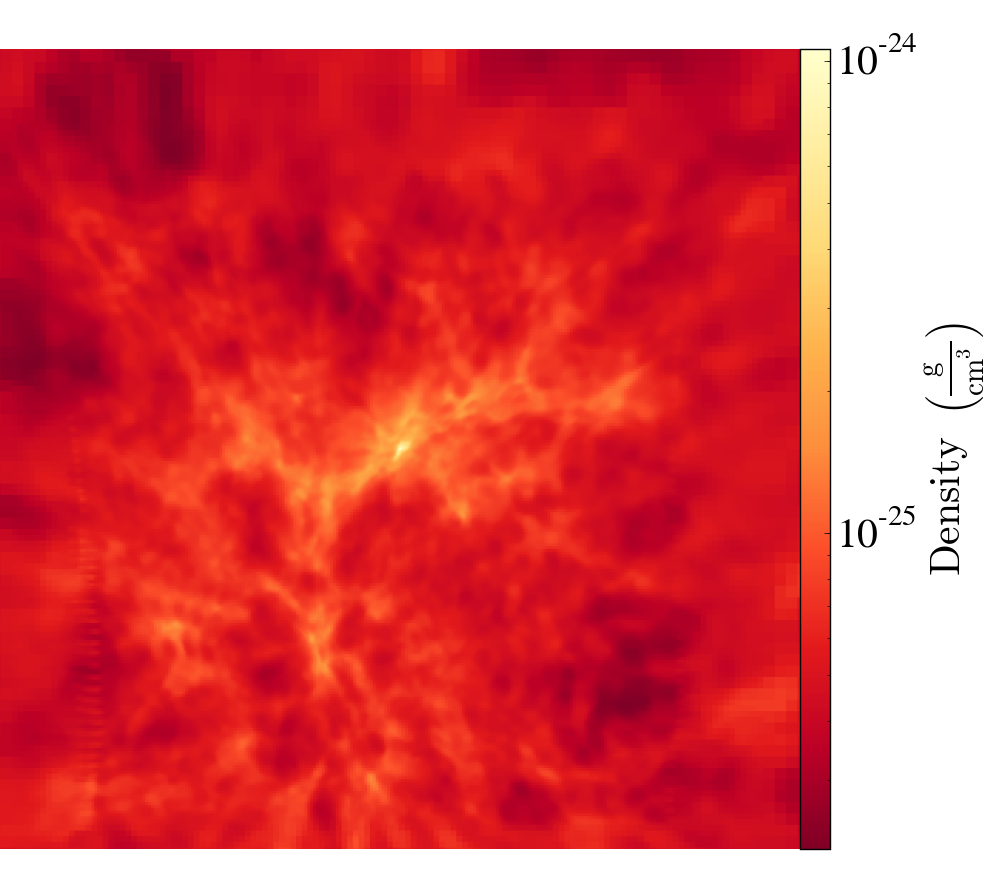
\includegraphics[height=7.9cm]{../kuvat/amr-nogrid.png}
   \end{subfigure}
   \caption{Läpileikkaus $100$ pc$^2$ alueesta Enzo-simulaatiosta (julkaisua Regan et al. 2015 varten), jonka hilojen rajat näkyvillä (vasen kuva) sekä ilman niitä (oikea kuva). Kiinnostavammilla alueilla solut ovat pienempiä. Resoluution heikentyminen simulaation reuna-alueilla sijaitsevissa suuremmissa ja harvemmissa hiloissa on selvästi nähtävissä oikeanpuoleisessa kuvassa.}\label{fig:enzogrid} %TODO onko tuossa Regan et al. 2015 mitään järkeä?
\end{figure}
	
Kullakin hilalla juurihilaa lukuun ottamatta on vanhempi, joka sisältää hilan kokonaan. Yhdellä hilalla voi olla useita lapsia, mutta aina vain yksi vanhempi. Näin hilat muodostavat puumaisen rakenteen. Tavallisesta puita koskevasta nimeämiskäytännöstä poiketen sisaruksiksi kutsutaan kaikkia niitä hiloja, joiden resoluutio on sama eli ne sijaitsevat puussa samalla tasolla. \cite{enzo}
	
Hienompia hiloja luotaessa valitaan hilan solujen koko siten, että hila rajoittuu reunoistaan vanhempansa solujen tahkoihin. Lisäksi solun vanhemman sivun pituuden tulee olla jokin monikerta solun sivun pituudesta. \cite{enzo}

Kukin hila koostuu varsinaisen datan tallettavien aktiivisten vyöhykkeiden (\textit{active zone}) lisäksi haamuvyöhykkeistä (\textit{ghost zone}), joita käytetään laskennassa tarvittavien aktiivisten vyöhykkeiden arvojen päivittämiseen tarvittavien naapurisolujen varastoimiseen väliaikaisesti. Hydrodynamiikkaa varten haamuvyöhykkeitä on kolme kerrosta kullakin aktiivisen vyöhykkeen tahkolla. Haamuvyöhykkeiden arvot saadaan interpoloimalla hilan vanhemmasta tai kopioimalla sisaruksista.\cite{arxivenzo, enzo}

\subsection{Numeerinen ratkaiseminen} %TODO retardi otsikko
Enzo tarkastelee kutakin hilaa omana ongelmanaan ratkaisten tarvittavat yhtälöt kullekin hilalle erikseen käyttäen reunaehtoina haamuvyöhykkeistä saatavia arvoja. Aluksi määritetään halutun tarkkuuden saavuttamiseksi tarvittava aika-askel kullekin puun tasolle. Tämän jälkeen aletaan tasoja käydä läpi W-syklin mukaisesti (kuva \ref{fig:w-cycle}). \cite{enzo} %TODO W-syklin mukaisesti?

W-syklissä kunkin tason kaikille hiloille lasketaan aluksi niiden tila yhden aika-askeleen kuluttua. Laskeminen aloitetaan juurihilasta se etenee tasoittain, kunnes kaikki AMR-puun lehdet on käsitelty. Seuraavaksi puun alimmalla tasolla olevia hiloja edistetään niin monta aika-askelta kuin tarvitaan, jotta saavutetaan ylempi taso, jonka hiloja edistetään myös yhden aika-askeleen verran. Tämän jälkeen alimman tason hiloja edistetään taas, kunnes ylempi taso on jälleen saavutettu. \cite{enzo}

Hilojen edistämistä jatketaan näin, edistäen aina tason $l$ hiloja, kunnes ne saavuttavat tason $l-1$ hilat, jolloin tason $l-1$ hiloja edistetään jälleen yhden aika-askeleen verran. Näin seuraava aika-askel lasketaan aina sille tasolle, jolla aikaa simulaation alusta on kulunut vähiten. Kun hiloja on edistetty niin pitkälle, että on jälleen aika edistää tason 0 hilaa, sykli alkaa alusta. \cite{enzo}

\begin{figure}
   \centering
   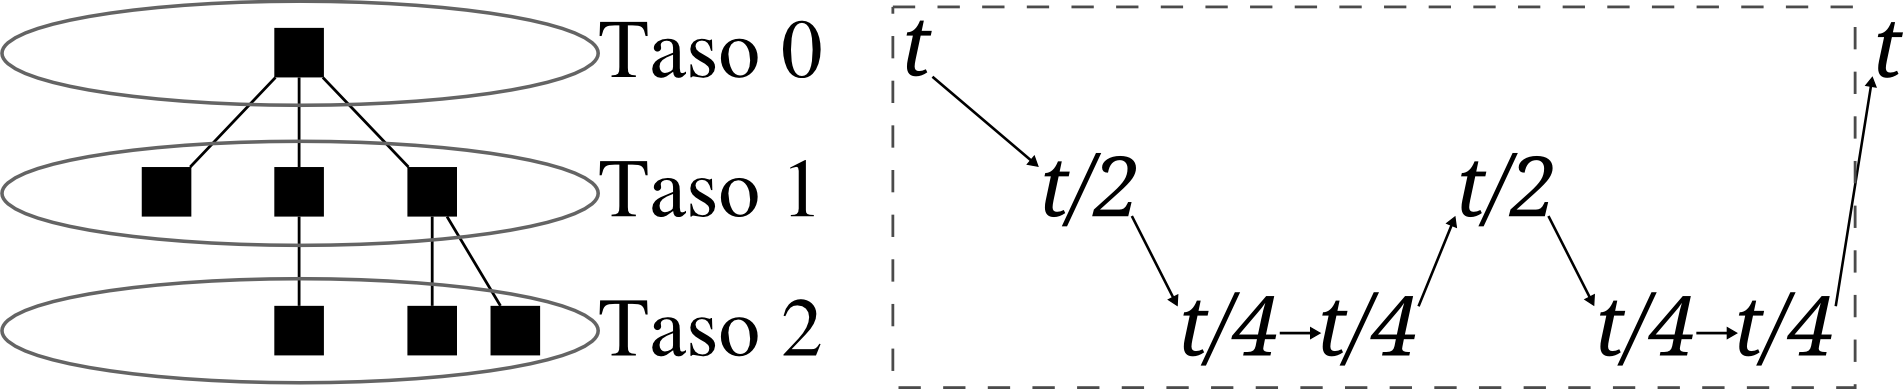
\includegraphics[width=\textwidth]{../kuvat/W-cycle.png}
   \caption{Vasemmalla kolmitasoinen hierarkia hiloja ja oikealla niiden läpikäyntijärjestys W-syklissä ja aika-askeleiden pituudet kun oletetaan, että tason $l+1$ aika-askel on puolet tason $l$ aika-askeleen pituudesta ja tason $0$ aika-askeleen pituus on $t$. Katkoviivalla on erotettu vaiheet, joiden jälkeen kunkin tason hilat ovat edenneet ajan $t$ verran eli ollaan jälleen alkutilannetta vastaavassa tilanteessa, jolloin sykli alkaa uudelleen.}\label{fig:w-cycle} %TODO W-syklissä?
\end{figure}

%Siksi AMR-simulaatioissa 

%Esimerkiksi kuvassa \ref{fig:enzogrid} nähdään, kuinka tiheämmillä alueilla käytetään pienempiä 


\section{\yt}
\yt\ on avoimen lähdekoodin Python-paketti, joka on mahdollistaa simulaatiotulosten helpon lukemisen, analysoinnin ja visualisoinnin. Kehitystyön alkuvaiheessa se sopi käytettä\-väksi vain Enzo-simulaatioiden kanssa, mutta nykyään sillä voidaan suoraan lukea sekä muiden AMR-simulaatioiden (kuten RAMSES tai BoxLib) että N kappaleen simulaatioiden (esimerkiksi Gadget) tuloksia. \cite{yt}

\subsection{Käyttäjän ja simulaatiodatan välinen rajapinta}
\yt\ abstrahoi hyvin voimakkaasti lukemansa datan, jolloin käyttäjä voi keksittyä fysikaalisiin rakenteisiin, joita simulaatio edustaa. Kun käyttäjä on ladannut simulaatiodatan, voi siitä tarkastella esimerkiksi pallomaista aluetta antamalla alueen keskustan koordinaatit ja pallon säteen ilman, että käyttäjän tarvitsee esimerkiksi etsiä niitä hiloja, jotka kattavat alueen parhaalla mahdollisella resoluutiolla tai tietää, missä tiedostoissa data on tallennettuna. Lisäksi \yt\ huolehtii yksikkömuunnoksista. \cite{yt}

Koska dataa käsitellään abstrakteina olioina, voidaan samaa ohjelmaa käyttää myös eri simulaatioista saadun datan kanssa vaihtamalla luettavaa datasettiä. Esimerkiksi alla oleva koodisegmentti lataa sijainnissa ''data'' olevan simulaation muistiin ja plottaa sen jälkeen sivultaan 500 kpc olevan alueen poikkileikkauksen tiheyden ja tallentaa sen. Ohjelma ei ota kantaa luettavan datan muotoon, ja onkin siksi helposti käytettävissä minkä tahansa \yt :n tukeman datasetin kanssa ainoastaan vaihtamalla datasettiä ladattaessa annettavaksi parametriksi halutun datan sijainti. \cite{yt, cookbook}

\begin{minipage}{\textwidth}
\lstset{style=python}
\begin{lstlisting}
import yt
dataset = yt.load("data")
plot = yt.SlicePlot(dataset, "x", "density", width = (500, "kpc"))
plot.save("slice.png")
\end{lstlisting}
\end{minipage}

Simulaatiodatassa olevien tietojen lisäksi \yt\ pystyy laskemaan datasta myös monia muita suureita kuten vaikkapa kulmaliikemäärän, maksimi- ja minimiarvoja sekä niiden sijainteja tai massakeskipisteen sijainnin. Lisäksi käyttäjän on mahdollista luoda omia kenttiä. Alla on \yt :n dokumentaatiosta\footnote{\url{http://yt-project.org/doc/developing/creating_derived_fields.html}} mukailtu esimerkki koodinpätkästä, jolla lisättäisiin paine \yt :n tuntemien kenttien joukkoon. Uudelle kentälle määritellään nimen ja funktion lisäksi myös yksikkö. \cite{yt, derivedfields}

\begin{minipage}{\textwidth}
\lstset{style=python}
\begin{lstlisting}
def _pressure(field, data):
    return (data.ds.gamma - 1.0) * data["density"] * data["thermal_energy"]
yt.add_field("pressure", function=_pressure, units="dyne/cm**2")
\end{lstlisting}%TODO gamma? specific heat ratio? keksi parempi kenttä? vaihda ainakin yksiköt
\end{minipage}

Laskettujen suureidin laskemisen jälkeen \yt\ tarjoaa laajan valikoiman työkaluja tulosten visualisointiin. Aiemmin esiteltyjen halkileikkausten lisäksi \yt :llä voi luoda muun muassa erilaisia profiileja, painottamattomia tai painotettuja projektioita tai 3D-renderöintejä. \cite{yt}

\subsection{Rinnakkaistaminen}
Usein visualisoitavaa dataa on hyvin paljon ja tietokoneiden kehittyessä sen määrä edelleen lisääntyy, jolloin rinnakkaislaskennan käyttö myös datan analysoinnissa tulee tärke\-äm\-mäksi ja tärkeämmäksi. \yt\ käyttää \texttt{mpi4py}-moduulia mahdollistaakseen datan rinnakkaisen käsittelyn niissä tehtävissä, jotka ovat helposti rinnakkaistettavissa. Tälläisiä ovat esimerkiksi tehtävät, joissa simuloitava alue voidaan jakaa eri prosessorien kesken. Muun muassa projistointi on mahdollista toteuttaa siten, että kukin prosessori laskee tietyn joukon näkösäteitä, jotka lopuksi yhdistetään yhdeksi plotiksi.\cite{yt}

Käyttäjä voi ottaa rinnakkaistuksen käyttöön ohjelmassaan yksinkertaisesti lisäämällä ohjelmansa alkuun rivin \texttt{yt.enable\_parallelism()}. Lisäksi ohjelman suorittamiseen on luonnollisesti käytettävä \texttt{mpirun}-komentoa. Tällöin \yt\ osaa rinnakkaistaa esimerkiksi projektioiden, poikkileikkausten, profiilien ja 3D-renderöintien luonnin sekä halojen etsimisen. Tarvittaessa joitain operaatioita voidaan suorittaa sarjallisesti esimerkiksi tarkastamalla funktion \texttt{yt.is\_root()} palauttama arvo, joka palauttaa arvon \texttt{True} jos kutsuvalla prosessorilla on MPI rank 0, muuten \texttt{False}. \cite{yt, parallel}

\yt\ pystyy käsittelemään myös useita datasettejä tai objekteja rinnakkain. Käyttämällä jokerimerkkejä kuten \texttt{*} ja \texttt{?} dataa ladattaessa, voidaan kerralla ladata useita datasettejä tai objekteja käsiteltäväksi rinnakkain. Tämän jälkeen ne voidaan käydä läpi käyttäen \texttt{piter()}-funktiota, joka jakaa käsiteltävät oliot prosessorien kesken. \cite{parallel}%TODO objekteja käytettäessä lataus tehdään oikeastaan vasta myöhemmin http://yt-project.org/doc/analyzing/parallel_computation.html#parallelizing-over-multiple-objects

\subsection{Visualisoinnin upottaminen simulaatiokoodiin}
Vaikka simulaation tila voidaan tarvittaessa tallentaa vaikka jokaisen aika-askeleen jälkeen, on prosessi hidas ja vaatii suuria tai pitkäkestoisia simulaatioita ajettaessa kohtuuttoman paljon levytilaa. Python/C API mahdollistaa muistissa olevan datan antamisen Python-tulkille simulaation sisällä. \yt\ puolestaan tarjoaa API:n jolla simulaation informaatio voidaan välittää analyysipaketille ja \yt :tä voidaan käyttää ajossa olevan simulaation analysointiin. \cite{yt}

Kun simulaation outputteja ei tarvitse tallentaa visualisointia varten, voidaan kuvia tai plotteja tallentaa huomattavasti useammin ja saavutetaan huomattavasti parempi tarvittavan tallennustilan ja tallennetun hyödyllisen informaation määrän suhde, sillä simulaation outputin koko liikkuu usein gigatavujen luokassa kun taas esimerkiksi kuvat ovat vain joitain kymmeniä tai satoja kilotavuja. Tyypillisesti dataa redusoidaan voimakkaasti joka tapauksessa, joten alkuperäisen outputin tallentaminen ei välttämättä ole mielekästä niin usein kuin esimerkiksi sulavan animaation tuottamiseksi on tarpeen. \cite{yt}

\subsection{Kuvien luominen}
\yt\ piilottaa paljon plottien luomiseen tarvittavista esimerkiksi datan tallennusmuotoon tai numeeristen arvojen väreiksi muuttamiseen liittyvistä toimista. On kuitenkin ohjelman suorituskyvyn ja tuotettujen kuvien ymmärtämisen kannalta tärkeää ymmärtää jonkin verran myös \yt :n toimintaa. Alla on eritelty muutamien kuvien luomisen mekaniikkaa hieman käyttäjälle näytettävää pintaa syvemmältä.

\subsubsection{Läpileikkaukset ja projektiot}
Läpileikkausten ja projektioiden luominen \yt :llä on pääpiirteissään melko samanlaista, tärkeimpänä erona käsiteltävän data-alueen laajuus. Läpi\-leikkausten luominen on tyypillisesti melko nopeaa, sillä niiden tekemiseksi täytyy käydä läpi vain ohut viipale datasetistä. Plotti luodaan hakemalla ensin tarvittava data datasetistä suurimmalla mahdollisella resoluutiolla \texttt{Fixed\-Resolution\-Buffer}-luokkaan (FRB), josta muodostetaan kuva käyttäjän määrittelemästä kohdasta. Samaa FRB:tä voidaan käyttää useiden kuvien renderöintiin mikäli kuvaa halutaan esimerkiksi zoomata tai panoroida. Tämä nopeuttaa kuvien luomista hieman. \cite{sliceproj}

Projektioiden luominen \yt :llä onnistuu pääpiirteissään samalla tavoin kuin läpi\-leik\-kaus\-ten\-kin. Projektiota luotaessa täytyy käydä läpi koko näkösäde kutakin lopullisen kuvan pikseliä kohden, joten niiden luominen on tyypillisesti hieman hitaampaa kuin läpi\-leikkausten. Ne tuovat kuitenkin usein läpileikkauksia paremmin esiin näkösäteen suunnassa laajempia rakenteita. Kuten läpileikkauksiakin, myös projektioita voi tehdä myös muissa kuin simulaation koordinattiakselien suunnissa käyttäen \texttt{OffAxisProjectionPlot}-luokkaa. \cite{sliceproj}

\begin{sloppypar}Projektiota luotaessa pikselien arvot voidaan määrittää usealla eri tavalla. Yleisimpiä näistä ovat painotettu ja painottamaton integrointi, joka määritetään asettamalla \texttt{method=integrate}. Mikäli \texttt{weight\_field}-parametria ei ole asetettu, lasketaan painottamaton keskiarvo yhtälön \ref{equ:unweighted} mukaisesti integroimalla haluttu kenttä $f(x)$ näkösäteen $\hat{n}$ suunnassa tutkittavan alueen yli. Tällöin projisoidun kentän yksikkö on alkuperäisen kentän yksikkö kerrottuna pituusyksiköllä. Mikäli \texttt{weight\_field} on määritelty, lasketaan kentän painotettu keskiarvo yhtälön \ref{equ:weighted} mukaisesti. Tällöin myös yksikkö säilyy projisoinnissa samana. \cite{sliceproj}
\begin{equation}\label{equ:unweighted}
	g(X) = {\int\ {f(x)\hat{n}\cdot{dx}}}
\end{equation}
\begin{equation}\label{equ:weighted}
	g(X) = \frac{\int\ {f(x)w(x)\hat{n}\cdot{dx}}}{\int\ {w(x)\hat{n}\cdot{dx}}}
\end{equation}
\end{sloppypar} 

Muita mahdollisia projisointitapoja ovat ovat \texttt{mip} ja \texttt{sum}. Näistä ensimmäinen valitsee projisoitavan kentän maksimiarvon kullakin näkösäteellä ja jälkimmäinen integroinnin sijaan summaa kentän arvot näkösäteellä ottamatta huomioon kuljetun polun pituutta. Siksi \texttt{sum} sopiikin käytettäväksi vain sellaisten gridien kanssa, joiden solut ovat vakiokokoisia, sillä muuten syntyvä kuva saattaa olla hyvin epäfysikaalinen. Kumpikin säilyttää alkuperäisen kentän yksiköt. \cite{sliceproj, projection}

\subsubsection{3D}
\yt\ tarjoaa myös mahdollisuuden kolmiulotteisten rakenteiden tarkastelemiseen tilavuusrenderöimällä. Kuten kaksiulotteisissakin ploteissa myös tilavuusrenderöinnissä voidaan käyttää mitä tahansa simulaatiodatan kenttää, jolloin esimerkiksi katselusuuntaa kääntä\-mällä tai zoomaamalla kohti kiinnostavia alueita voidaan simulaation kiinnostavia piirteitä tuoda esiin joissain tilanteissa havainnollisemmin kuin läpileikkauksilla tai projektioilla. \cite{volume}

Tilavuusrenderöintiä varten on ensin luotava color transfer function, %TODO mikä suomeksi?
jonka perusteella määritetään tarkasteltavan tilavuuden emissio ja absorptio kussakin RGBA-väri\-järjes\-telmän kaistassa. Ne voi määrätä mikä tahansa simulaation kenttä joko painottamattomana tai painotettuna toisella kentällä. Täten color transfer function määrää kunkin pisteen värin paikan funktiona siten, että $f(v) \rightarrow (r, g, b, a)$. \cite{volume}

Seuraavaksi luodaan \texttt{camera}-olio, jolloin datalohkot jaetaan kuvattavan alueen täysin kattaviin ''tiiliin'' (\textit{bricks}), joihin valitaan parhaan mahdollisen resoluution data jokaisesta pisteestä. Nämä tiilet järjestetään näkösäteen suunnassa takaa eteen, jotta ne on helppo käydä läpi siinä järjestyksessä, jossa silmään saapuva säde kohtaa ne. Seuraavaksi luodaan kuvatason kanssa yhdensuuntainen taso säteitä kuvattavan alueen perälle alkuarvolla nolla. Näitä säteitä liikutetaan kohti katsojaa ja pikselien arvot päivitetään kullakin askeleella. \cite{volume}

\begin{sloppypar}
Kullekin tiilelle lasketaan, mitkä säteet leikkaavat sen. Kustakin säteestä otetaan \texttt{sub\_samples}-parametrilla määrättävä määrä näytteitä (oletusarvoisesti 5) ja arvot näytteenottokohdissa lasketaan solun kärkien arvoista trilineaarisella interpoloinnilla. Tämän jälkeen kussakin pisteessä lasketaan transfer function arvo, jolloin saadaan emission $j$ ja absorption $\alpha$ voimakkuus kussakin kaistassa. Näiden perusteella kullekin pikselille lasketaan uusi arvo ottaen huomioon säteen kulkema matka. Pikselin uusi arvo $v^{n+1}$ kaistassa $i$ saadaan pikselin aiemman arvon $v^n$ perusteella yhtälöstä \ref{equ:3d}, jossa $\Delta s$ on säteen kulkema matka näytteenottopisteiden välillä.
\begin{equation}\label{equ:3d}
v^{n+1}_{i} =  j_{i}\Delta s + (1 - \alpha_{i}\Delta s )v^{n}_{i}
\end{equation}
\end{sloppypar}

\section{Oma työ}
Aloitin \yt :hen tutustumisen selaamalla dokumentaatiota sekä cookbookia\footnote{\url{http://yt-project.org/docs/3.1/cookbook/}} ja ensin kopioimalla ja sittemmin muokkaamalla siellä annettuja malliohjelmia käyttäen esimerkkidataa. Tutustuin tarkimmin halkileikkauksiin, projektioihin ja 3D-renderöinteihin sekä muun muassa niiden akselien tekstien ja jaotuksen tai väriskaalojen muokkaamiseen. Lisäksi kokeilin \yt :n soveltamista animaatioiden tekemiseen.

Opittuani perusasiat aloin soveltaa niitä tutkimusryhmämme tuottamaan dataan kaasupilven romahtamista suoraan mustaksi aukoksi koskevista simulaatioista (Regan et al. 2015). Samalla otin selvää \yt :n tarjoamista mahdollisuuksista usean plotin yhdistämiseksi yhteen kuvaan. Kun samaan kuvaan halutaan useantyyppisiä kuvia, tarvitaan \texttt{eps\_writer}-luokkaa. Sen tarjoama tuki profiileille oli kuitenkin puutteellinen, joten jouduin myös parantelemaan \yt :n lähdekoodia.

\subsection{Läpileikkaukset}
Aloitin tutustumalla \yt :n yksinkertaisimpiin plotteihin aloittaen läpileikkauksista. Niitä voidaan käyttää yksittäisinä näyttämään jokin alue simulaatiosta tai niitä voidaan renderöidä useita ja koostaa niistä animaatio. Esimerkiksi listing \ref{koodi:flythrough} lukee annetun datasetin ja tallentaa läpileikkauksen tiheyksistä simulaation tiheimmän kohdan ympäriltä sadasta kohdasta liikkuen z-akselia pitkin 1 kpc matkan. Esimerkissä tarkastellaan kohdetta koordinaattiakselin suunnasta, mutta läpileikkauksia voidaan luoda mielivaltaisesta suunnasta \cite{sliceproj}.

Lisäksi plotin väripalkin alueeksi asetetaan \SI{3e-26}{} -- \SI{2.5e-25}{\gram\per\cubic\centi\metre} ja colormapiksi hot\footnote{\url{http://yt-project.org/doc/visualizing/colormaps/}}. Lisäksi akseleilla käytettävän fontin kokoa kasvatetaan ja lopullinen kuva tallennetaan juoksevaa numerointia käyttäen. Neljä sadasta tuloksena saatavista plotista tasaisin välein valittua läpileikkausta on nähtävissä kuvassa \ref{fig:flythrough}.

\begin{minipage}{\linewidth}
\lstinputlisting[style=python, caption={Python-ohjelma, joka tallentaa 100 esimerkiksi animoitavaksi sopivaa framea, joissa sivultaan 3 kpc oleva läpileikkaus liikkuu simulaation z-akselin suunnassa läpi simulaation tiheimmän kohdan.}, label={koodi:flythrough}]{../python/flythrough.py}
\end{minipage}

\begin{figure}
   \centering
   \begin{subfigure}[b]{0.48\textwidth}
       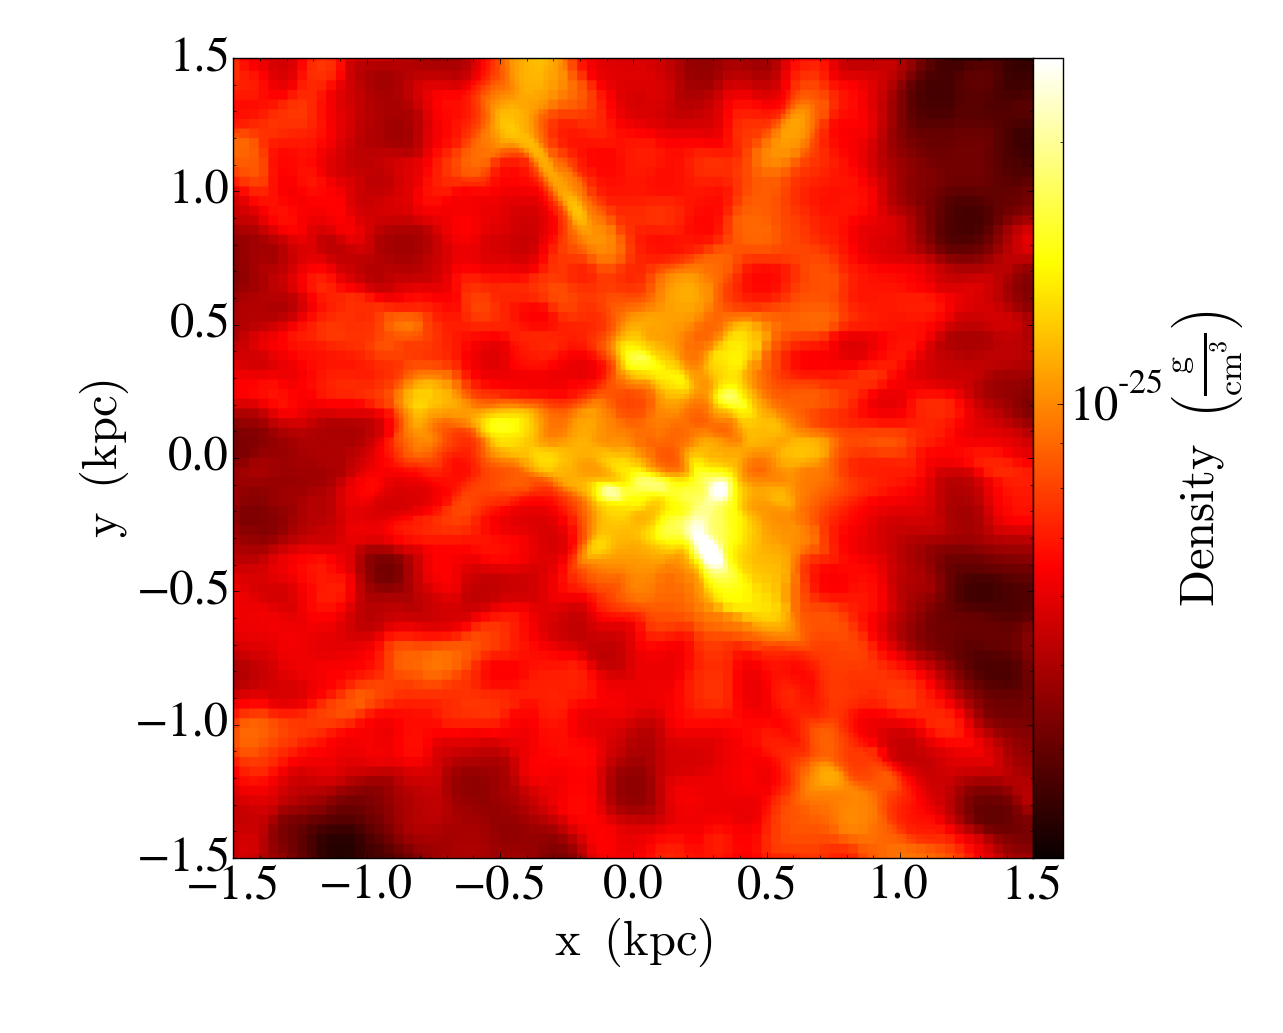
\includegraphics[width=\textwidth]{../kuvat/flythrough/0000.png}
   \end{subfigure}
   \begin{subfigure}[b]{0.48\textwidth}
       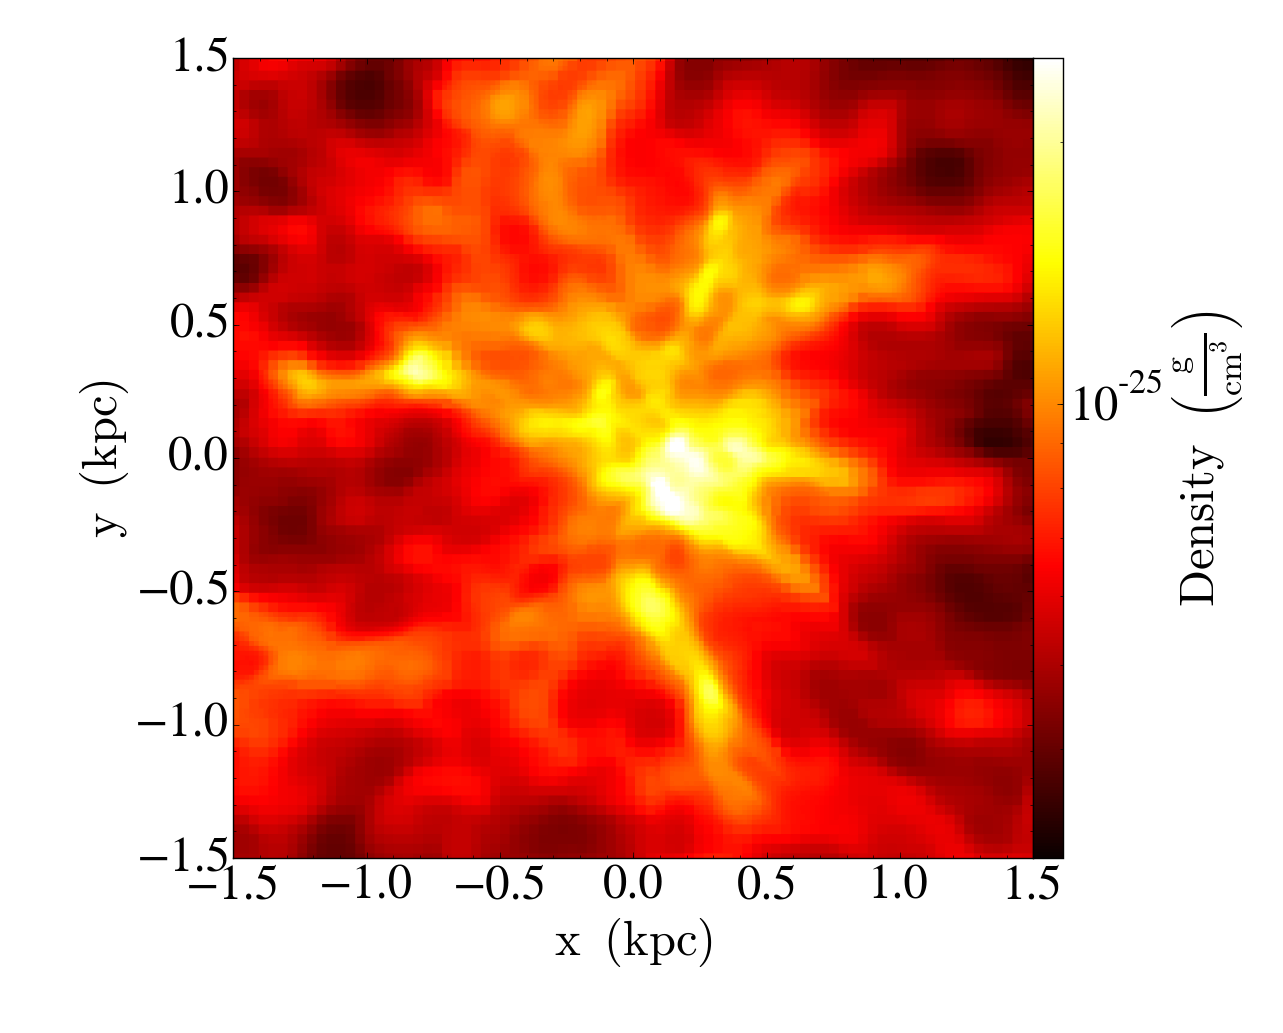
\includegraphics[width=\textwidth]{../kuvat/flythrough/0032.png}
   \end{subfigure}
   \begin{subfigure}[b]{0.48\textwidth}
       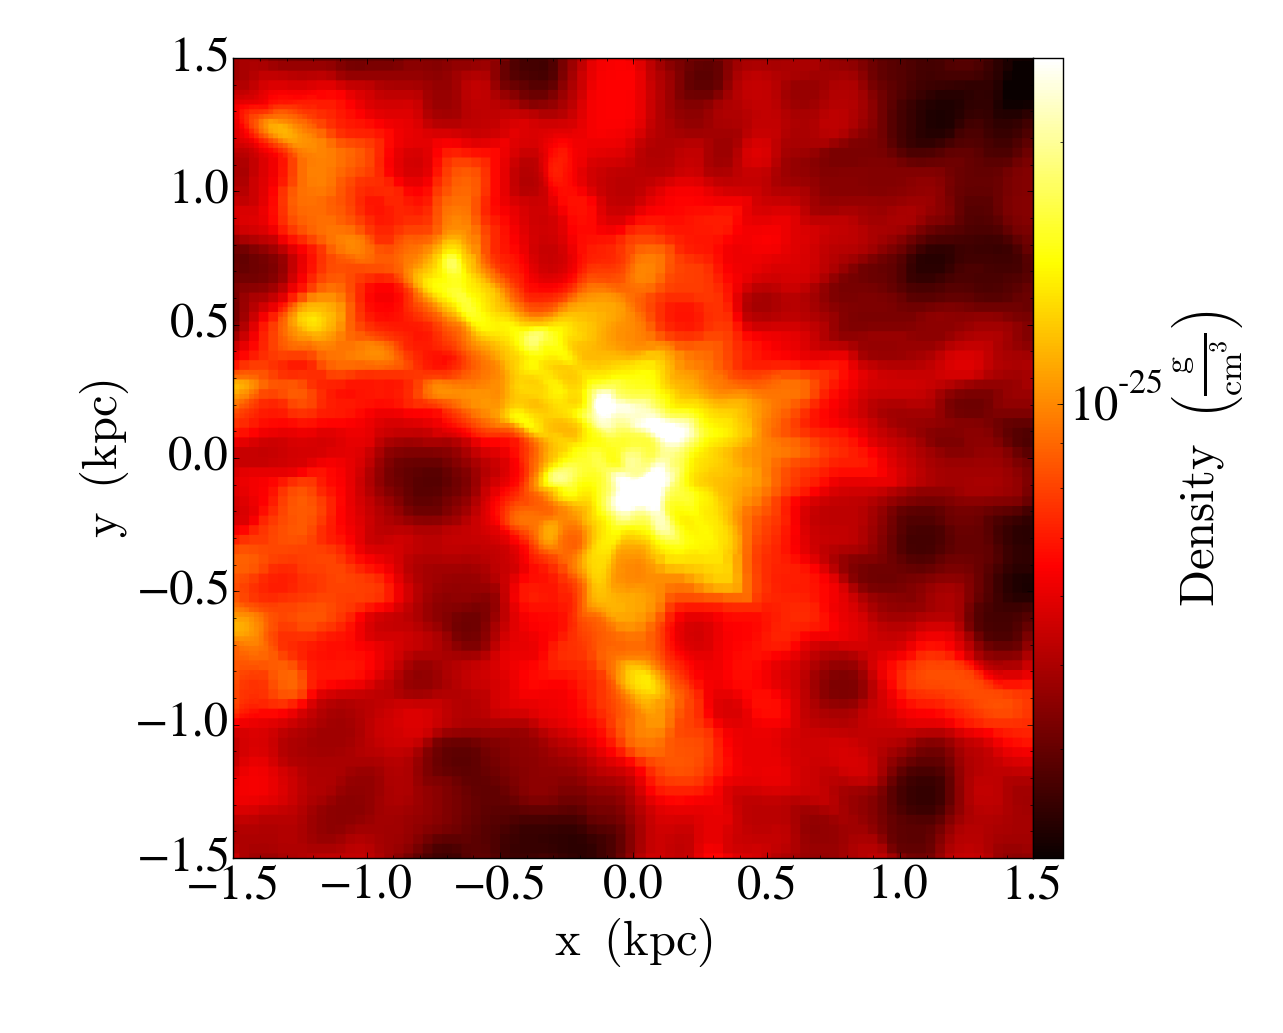
\includegraphics[width=\textwidth]{../kuvat/flythrough/0066.png}
   \end{subfigure}
   \begin{subfigure}[b]{0.48\textwidth}
       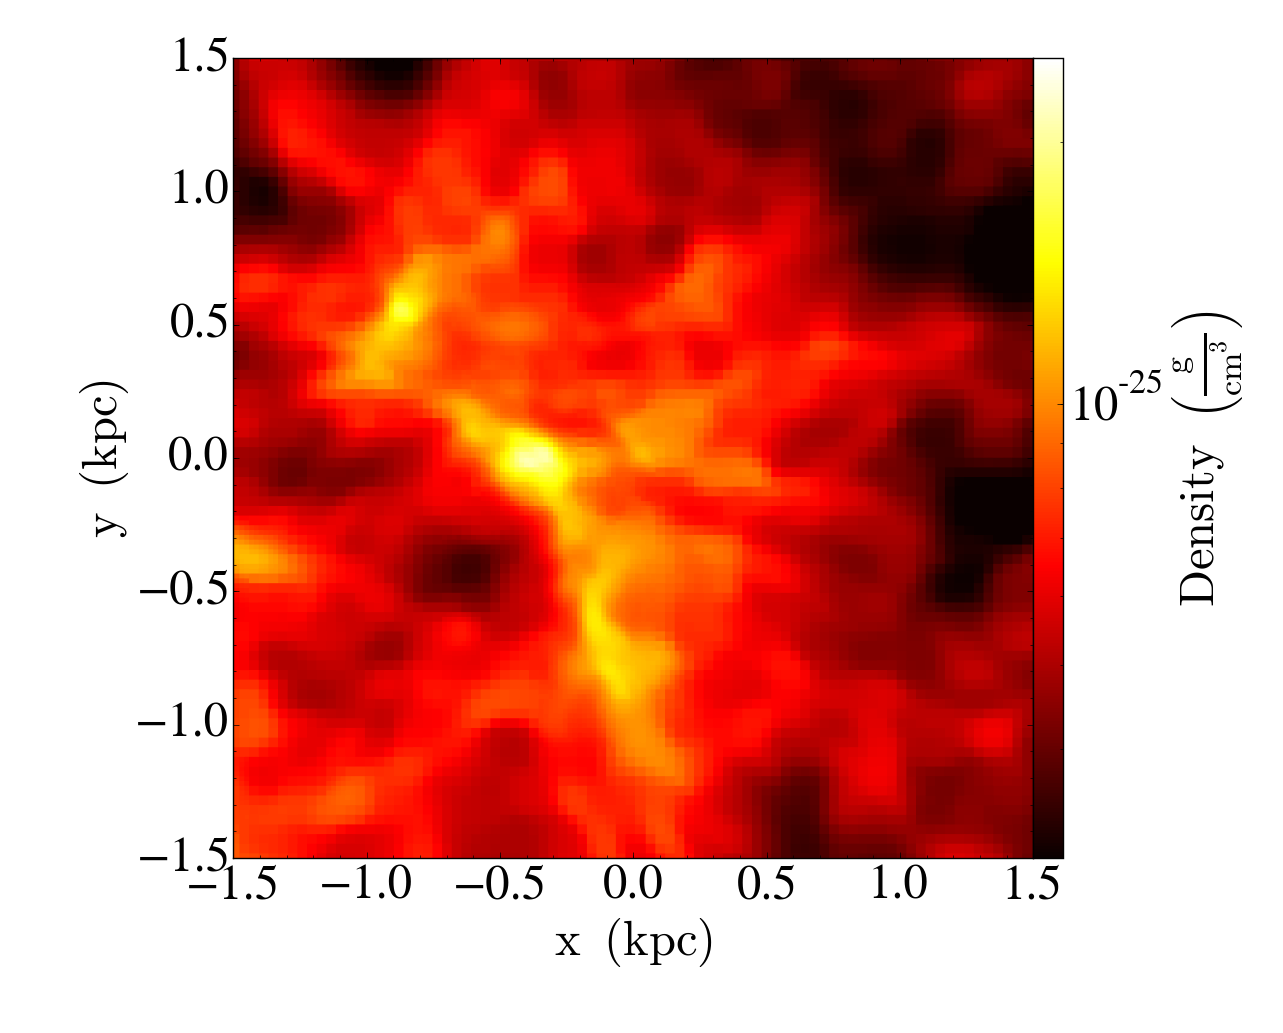
\includegraphics[width=\textwidth]{../kuvat/flythrough/0099.png}
   \end{subfigure}
   \caption{Neljä listingissä \ref{koodi:flythrough} esitetyn koodin tallentamista kuvista, kun se ajetaan julkaisua Regan et al. 2015 varten lasketulla datalla. Alueessa edetään syvemmälle riveittäin vasemmalta oikealle.}\label{fig:flythrough}
\end{figure}

\subsection{Projektiot}
%TODO kirjoita uusi alku

Listingissä \ref{koodi:projection} on esitetty yksinkertaisen projektion tallentava skripti. Se käyttää samaa simulaatiodataa kuin \ref{koodi:flythrough}, josta luodaan yksi projektio integroimalla $z$-akselin suuntaisen näkösäteen suunnassa. Skriptin tuottama kuva on nähtävissä kuvassa \ref{fig:projection}. Vertaamalla tätä kuvan \ref{fig:flythrough} läpileikkauksiin huomataan, että projisointi kadottaa näkösäteen suunnassa pienet yksityiskohdat, mutta projektiosta saa paremman kuvan suuremman skaalan rakenteista. Myös yksiköiden huomataan poikkeavan toisistaan, sillä projektiota luotaessa käytettiin painottamatonta integrointia.

%TODO ehkä myös jotain vähän lisää nyt kun osa on siirretty pois?

\begin{minipage}{\linewidth}
\lstinputlisting[style=python, caption={Yksinkertaisen projektion luomiseen soveltuva ohjelma. Käytetty alue datassa on sama kuin listingissä \ref{koodi:flythrough}, mutta useiden läpileikkausten sijaan luodaan yksi projektio.}, label={koodi:projection}]{../python/projection.py}
\end{minipage}

\begin{figure}
   \centering
   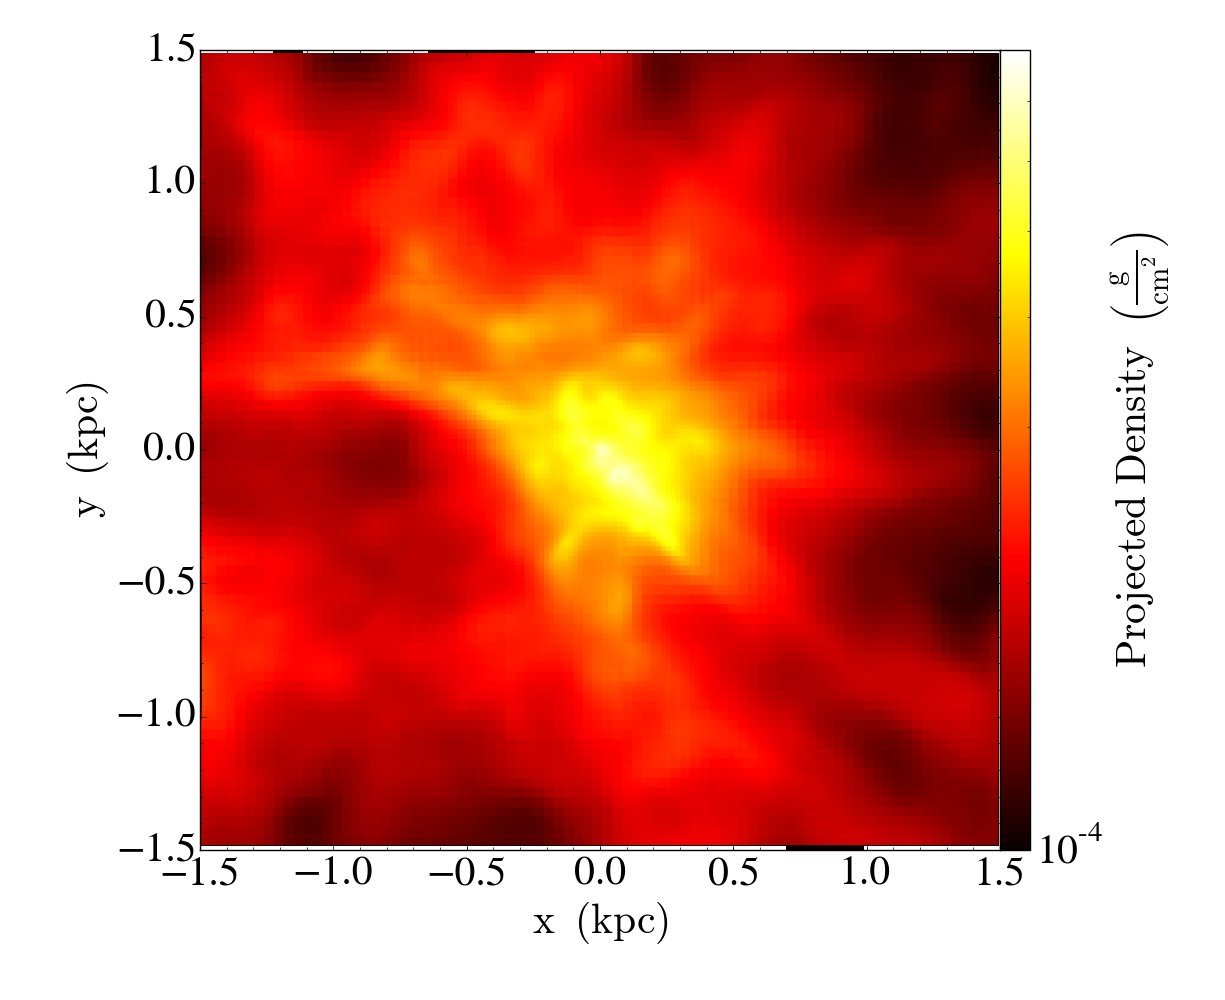
\includegraphics[width=.7\textwidth]{../kuvat/projection.png}
   \caption{Listingin \ref{koodi:projection} luoma projektio. Verrattuna kuvan \ref{fig:flythrough} läpileikkauksiin nähdään vähemmän yksityiskohtia, mutta projektio antaa paremman kokonaiskuvan koko alueesta kerralla.} \label{fig:projection}
\end{figure}

%TODO tällä haavaa päätelmiä on sekaisin omassa työssä

\subsection{3D}
Tilavuusrenderöinnit tuovat usein tutkittavan kohteen kolmiulotteisen rakenteen esiin projektioita ja läpileikkauksia intuitiivisemmin. Yksittäiset kuvat saattavat kuitenkin olla vaikeasti tulkittavia, sillä kohteiden etäisyyttä katsojasta on usein vaikeaa hahmottaa. Kuvista ja etenkin animaatioista on kuitenkin mahdollista saada erittäin näyttäviä. 

Liitteessä \ref{koodi:volume-spiraali} on esitetty skripti, jolla voidaan luoda framet animaatioon, jossa kamera sekä kiertää kohdetta että zoomaa sisään. Datan lataamisen jälkeen riveillä 10--13 etsitään datan tiheimmästä kohdasta korkeintaan 0,5 kpc päässä oleva paikka, jossa molekulaarisen vedyn osuus kaikesta vedystä on suurin hyödyntämällä \yt :n tarjoamia \texttt{find\_max}- ja \texttt{max\_location}-funktioita. Tämän jälkeen riveillä 16--19 määrätään tutkittavaksi alueeksi säteeltään 1 kpc pallo löydetyn suurimman molekulaarisen vedyn pitoisuuden kohdan ympärillä. Lisäksi täytyy määrittää kameran ja kuvan keskustan välinen vektori, kuvan leveys ja resoluutio. 

Kun tarvittavat parametrit on alustettu, voidaan camera-olio luoda. Kameran kuvaamiksi kentiksi asetetaan ainoastaan H2\_fraction. Lisäksi määritetään, että kuvassa näytetään ainoastaan aiemmin luodun 1 kpc säteisen pallon sisällä oleva aine, jolloin vältytään siltä riskiltä, että tutkittavan alan eteen tulee toinen huomattavasti molekulaarista vetyä sisältävä alue, joka estää tutkittavan alueen näkemisen.

Animaation luomiseksi käytetään kameran \texttt{zoomin}-funktiota, jolla on mahdollista iteroida haluttu zoomaus halutulla määrällä vakiokokoisia askelia. Esimerkin animaatiossa zoomauskertoimeksi on valittu 3 ja askelten määrä on valittu sellaiseksi, että kohde voidaan kiertää kerran 0,04 radiaanin askelin. Kierron toteuttamiseksi kameraa käännetään kunkin zoomauksen jälkeen. Tämän jälkeen \texttt{zoomin}-funktion palauttama kuva tallennetaan numeroituna.

%TODO ehkä siitä, että on suorituskyvyn kannalta oleellista käyttää yhtä kameraa ja kääntää ja liikuttaa sitä?

\subsection{Usean kuvaajan plotit}
\yt\ tarjoaa mahdollisuuden kuvaajien palauttamiseen taulukkona, joka voidaan edelleen käyttää esimerkiksi \texttt{matplotlib}in\footnote{\url{http://matplotlib.org/mpl_toolkits/axes_grid/api/axes_grid_api.html}} kanssa usean kuvaajan yhdistämiseksi samaan kuvaan. Tähän on kuitenkin myös apufunktio, jolle voidaan antaa suoraan joko kuvaajat tai jpg-kuvat, jotka asemoidaan haluttaessa väripalkkien kanssa ruudukkoon.

Liitteessä \ref{koodi:multiplot-simppeli} on nähtävillä \texttt{eps\_writer}iä hyödyntävä skripti, joka plottaa tiheyden ja lämpötilan 7 kpc leveällä alueella simulaation tiheimmän kohdan ympäriltä ja tallentaa ne sekä erikseen että yhdessä. Plotti, jossa molemmat ovat, on nähtävissä kuvassa \ref{fig:multiplot-simppeli}. Plotin muodostamista voidaan ohjata erilaisilla parametrina annettavilla lipuilla. Esimerkiksi esimerkissä on hyödynnetty parametreja \texttt{xaxis\_flags} ja \texttt{yaxis\_flags}, joilla asetetaan akselit plottien ulkoreunoille sekä parametria \texttt{cb\_location}, jolla väripalkit asetetaan kuvaajien yläpuolelle.

\begin{figure}
   \centering
   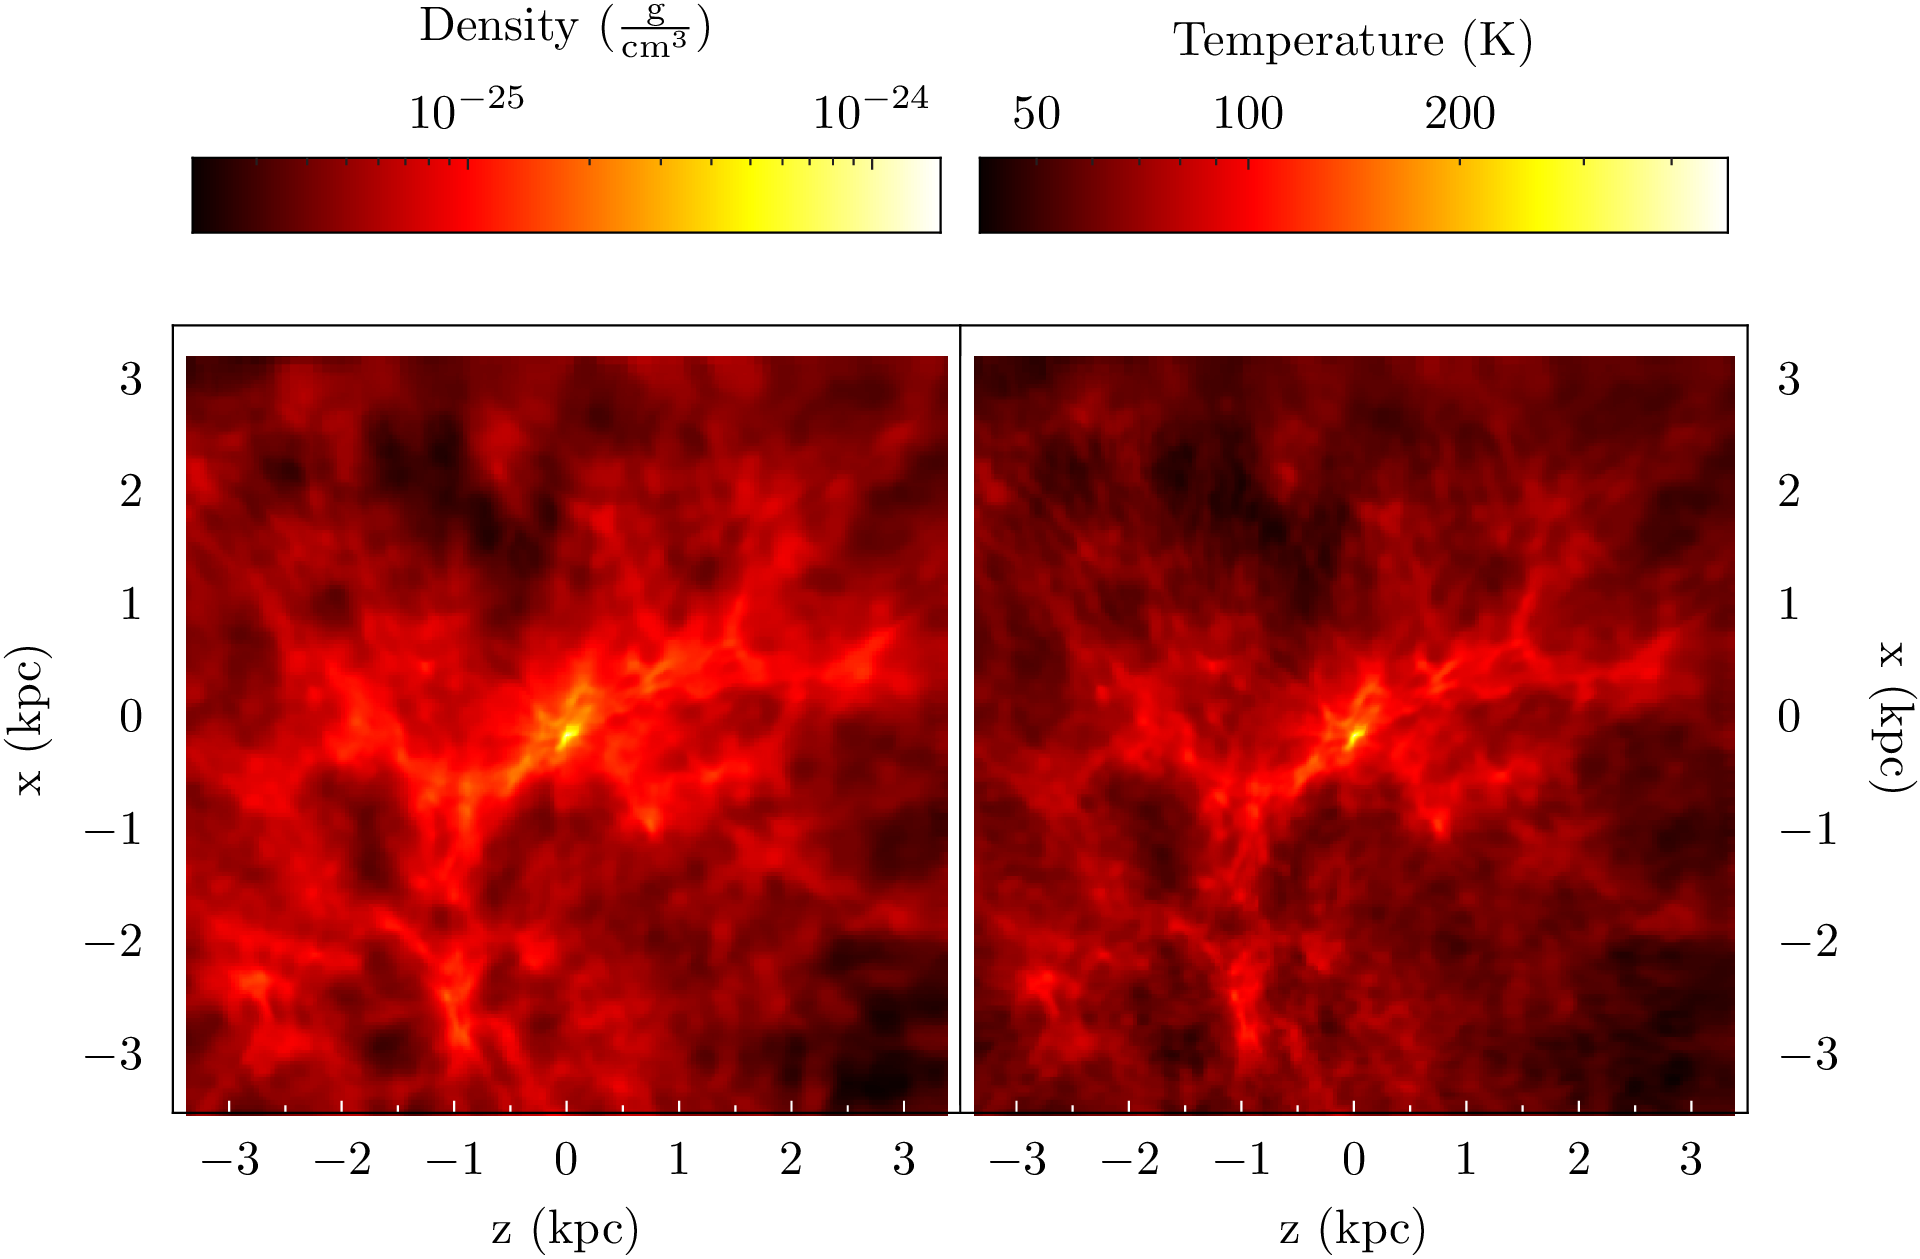
\includegraphics[width=\textwidth]{../kuvat/EPSMultiPlot.png}
   \caption{Liitteessä \ref{koodi:multiplot-simppeli} esitetyn skriptin tuottama kuva.} \label{fig:multiplot-simppeli}
\end{figure}

\yt\ on kuitenkin vielä kehittyvä paketti, mikä on selvästi huomattavissa \texttt{eps\_writer}-luokassa. %rajat, värit

\subsection{Muutokset \yt :n lähdekoodissa} %subsubsection?

%%%%% Sisältö loppuu, lähdeluettelo %%%%%
\bibliographystyle{plain}
\bibliography{lahteet} %TODO yt api on pienellä

\appendix
%\newpage
%\section{Läpilento} \label{koodi:kaanto-projection}
%\lstinputlisting[style=python]{../python/flythrough.py}
%\newpage
\section{3D-animaatio spiraaliradalla kohdetta lä\-hes\-tyen} \label{koodi:volume-spiraali}
\lstinputlisting[style=python]{../python/volume-spiraali.py}
\newpage
\section{Kaksi läpileikkausta samassa plotissa} \label{koodi:multiplot-simppeli}
\lstinputlisting[style=python]{../python/multiplot-simppeli.py}
\end{document}
